%
% ---------------------------------------------------------------
% Copyright (C) 2012-2018 Gang Li
% ---------------------------------------------------------------
%
% This work is the default powerdot-tuliplab style test file and may be
% distributed and/or modified under the conditions of the LaTeX Project Public
% License, either version 1.3 of this license or (at your option) any later
% version. The latest version of this license is in
% http://www.latex-project.org/lppl.txt and version 1.3 or later is part of all
% distributions of LaTeX version 2003/12/01 or later.
%
% This work has the LPPL maintenance status "maintained".
%
% This Current Maintainer of this work is Gang Li.
%
%

\documentclass[
 size=14pt,
 paper=smartboard,  %a4paper, smartboard, screen
 mode=present, 		%present, handout, print
 display=slides, 	% slidesnotes, notes, slides
 style=tuliplab,  	% TULIP Lab style
 pauseslide,
 fleqn,leqno]{powerdot}


\usepackage{cancel}
\usepackage{caption}
\usepackage{stackengine}
\usepackage{smartdiagram}
\usepackage{attrib}
\usepackage{amssymb}
\usepackage{amsmath} 
\usepackage{amsthm} 
\usepackage{mathtools}
\usepackage{rotating}
\usepackage{graphicx}
\usepackage{boxedminipage}
\usepackage{rotate}
\usepackage{calc}
\usepackage[absolute]{textpos}
\usepackage{psfrag,overpic}
\usepackage{fouriernc}
\usepackage{pstricks,pst-3d,pst-grad,pstricks-add,pst-text,pst-node,pst-tree}
\usepackage{moreverb,epsfig,subfigure}
\usepackage{color}
\usepackage{booktabs}
\usepackage{etex}
\usepackage{breqn}
\usepackage{multirow}
\usepackage{natbib}
\usepackage{bibentry}
\usepackage{gitinfo2}
\usepackage{siunitx}
\usepackage{nicefrac}
%\usepackage{geometry}
%\geometry{verbose,letterpaper}
\usepackage{media9}
\usepackage{animate}
%\usepackage{movie15}
\usepackage{auto-pst-pdf}

\usepackage{breakurl}
\usepackage{fontawesome}
\usepackage{xcolor}
\usepackage{multicol}



\usepackage{verbatim}
\usepackage[utf8]{inputenc}
\usepackage{dtk-logos}
\usepackage{tikz}
\usepackage{adigraph}
%\usepackage{tkz-graph}
\usepackage{hyperref}
%\usepackage{ulem}
\usepackage{pgfplots}
\usepackage{verbatim}
\usepackage{fontawesome}


\usepackage{todonotes}
% \usepackage{pst-rel-points}
\usepackage{animate}
\usepackage{fontawesome}

\usepackage{listings}
\lstset{frameround=fttt,
frame=trBL,
stringstyle=\ttfamily,
backgroundcolor=\color{yellow!20},
basicstyle=\footnotesize\ttfamily}
\lstnewenvironment{code}{
\lstset{frame=single,escapeinside=`',
backgroundcolor=\color{yellow!20},
basicstyle=\footnotesize\ttfamily}
}{}


\usepackage{hyperref}
\hypersetup{ % TODO: PDF meta Data
  pdftitle={Presentation Title},
  pdfauthor={Gang Li},
  pdfpagemode={FullScreen},
  pdfborder={0 0 0}
}


% \usepackage{auto-pst-pdf}
% package to show source code

\definecolor{LightGray}{rgb}{0.9,0.9,0.9}
\newlength{\pixel}\setlength\pixel{0.000714285714\slidewidth}
\setlength{\TPHorizModule}{\slidewidth}
\setlength{\TPVertModule}{\slideheight}
\newcommand\highlight[1]{\fbox{#1}}
\newcommand\icite[1]{{\footnotesize [#1]}}

\newcommand\twotonebox[2]{\fcolorbox{pdcolor2}{pdcolor2}
{#1\vphantom{#2}}\fcolorbox{pdcolor2}{white}{#2\vphantom{#1}}}
\newcommand\twotoneboxo[2]{\fcolorbox{pdcolor2}{pdcolor2}
{#1}\fcolorbox{pdcolor2}{white}{#2}}
\newcommand\vpspace[1]{\vphantom{\vspace{#1}}}
\newcommand\hpspace[1]{\hphantom{\hspace{#1}}}
\newcommand\COMMENT[1]{}

\newcommand\placepos[3]{\hbox to\z@{\kern#1
        \raisebox{-#2}[\z@][\z@]{#3}\hss}\ignorespaces}

\renewcommand{\baselinestretch}{1.2}


\newcommand{\draftnote}[3]{
	\todo[author=#2,color=#1!30,size=\footnotesize]{\textsf{#3}}	}
% TODO: add yourself here:
%
\newcommand{\gangli}[1]{\draftnote{blue}{GLi:}{#1}}
\newcommand{\shaoni}[1]{\draftnote{green}{sn:}{#1}}
\newcommand{\gliMarker}
	{\todo[author=GLi,size=\tiny,inline,color=blue!40]
	{Gang Li has worked up to here.}}
\newcommand{\snMarker}
	{\todo[author=Sn,size=\tiny,inline,color=green!40]
	{Shaoni has worked up to here.}}

%%%%%%%%%%%%%%%%%%%%%%%%%%%%%%%%%%%%%%%%%%%%%%%%%%%%%%%%%%%%%%%%%%%%%%%%
% title
% TODO: Customize to your Own Title, Name, Address
%
\title{New York City Taxi Trip Duration Project}
\author{
 Qin Zhang 
\\Chongqing Technology and Business University
}
\date{2022/8/21}


% Customize the setting of slides
\pdsetup{
% TODO: Customize the left footer, and right footer
rf=\href{http://www.tulip.org.au}{
Last Changed by: \textsc{Qin Zhang}\ \gitVtagn-\gitAbbrevHash\ (\gitAuthorDate)
},
cf={New York City Taxi Trip Duration},
}


\begin{document}

\maketitle

%\begin{slide}{Overview}
%\tableofcontents[content=sections]
%\end{slide}


%%==========================================================================================
%%
\begin{slide}[toc=,bm=]{Overview}
\tableofcontents[content=currentsection,type=1]
\end{slide}
%%
%%==========================================================================================


\section{Project Description}


%%==========================================================================================
%%

\begin{slide}{Project Description}

\begin{itemize}
\item The competition dataset is based on the 2016 NYC Yellow Cab trip record data made available in Big Query on Google Cloud Platform. The data was originally published by the NYC Taxi and Limousine Commission (TLC). The data was sampled and cleaned for the purposes of this playground competition. Based on individual trip attributes, participants should predict the duration of each trip in the test set.

\item The project provided \textcolor{orange}{1458644} pieces of effective data for the construction of machine learning model. The purpose of the project is to predict the \textcolor{orange}{trip-duration} time of passengers through "characteristics" such as pickup-datetime and dropoff-datetime.
\end{itemize}




%%==========================================================================================
\begin{note}
First, I will introduce the problem definition.
In the real life,
a teacher may be interested in the characteristics that
make one student obvious different from others.
Or,
NBA sports coaches would prefer to
know the advantages and disadvantages of one player.
Here, the player can be regarded as a query object.

For example, team A has five players,
each player has four features.
The NBA sports coaches may want to know the features of
player $1$ that are different from others.

The above example can be seen as outlying aspects mining.
The main purpose of outlying aspects mining is to identify
the outstanding features of the query object.



\end{note}
%%==========================================================================================

\end{slide}
%%
%%==========================================================================================



%%
%%==========================================================================================


\section{Data Description}


%%==========================================================================================
%%

%%==========================================================================================
%%page 3  fig-02
\begin{slide}{Data Description}


\begin{itemize}

\item
Data fields:

\begin{itemize}
\item
id : a unique identifier for each trip

\item
vendor-id : a code indicating the provider associated with the trip record

\item
pickup-datetime : date and time when the meter was engaged

\item
dropoff-datetime : date and time when the meter was disengaged

\item
passenger-count : the number of passengers in the vehicle (driver entered value)

\item
pickup-longitude : the longitude where the meter was engaged

\item
pickup-latitude : the latitude where the meter was engaged

\item
dropoff-longitude : the longitude where the meter was disengaged

\item
dropoff-latitude : the latitude where the meter was disengaged

\item
store-and-fwd-flag : This flag indicates whether the trip record was held in vehicle memory before sending to the vendor because the vehicle did not have a connection to the server - Y=store and forward; N=not a store and forward trip

\item
trip-duration : duration of the trip in seconds

\end{itemize}
\end{itemize}


%%==========================================================================================
\begin{note}
Based on the above example,
I will compare the differences
between outlying aspects mining and outlier detection.

Outlying aspects mining aims to
explain the distinctive aspects of the query object.
The query object may or may not be an outlier.
In contrast,
Outlier detection aims to discover all possible
outlying objects in the dataset.
Without explaining how and why they are different.

\begin{center}
\begin{tabular}{c| c c c c }
\toprule
%\centering
Player & \texttt{3PT\%}  & \texttt{FTA} & \texttt{FT\%} & \texttt{To} \\
\midrule
$P_1$
&  {$65$} &  {$4$} &  {$33$} &  {$8$} \\
$P_2$
&  {$78$} &  {$1$}&  {$65$}&  {$5$} \\
$P_3$
&  {$58$} &  {$6$} &  {$46$} &  {$3$} \\
$P_4$
&  {$68$} &  {$1.2$}&  {$85$}&  {$6.2$} \\
$P_5$
&  {$58$} &  {$6.2$} &  {$36$} &  {$3.4$}\\
\bottomrule
\end{tabular}
\end{center}

Let's go back to the NBA example,
in that example,
%two column words
the output of the outlying aspects mining may be
a combination of four features,
but the output of the outlier detection may be any of those five players.
\end{note}
%%==========================================================================================

\end{slide}
%%
%%==========================================================================================



%%==========================================================================================
%%
\begin{slide}[toc=,bm=]{Data Description}




\begin{table}[]
\setlength{\abovecaptionskip}{0pt}
\setlength{\belowcaptionskip}{10pt}
\setlength{\tabcolsep}{10pt} % Default value: 6pt
\renewcommand{\arraystretch}{1.5} % Default value: 1
\centering
\caption{Dataset description}
\resizebox{\textwidth}{!}{
\begin{tabular}{cccccccccccc}
\hline
\textbf{}  & \textbf{id} & \textbf{vendor\_id} & \textbf{pickup\_datetime} & \textbf{dropoff\_datetime} & \textbf{passenger\_count} & \textbf{pickup\_longitude} & \textbf{pickup\_latitude} & \textbf{dropoff\_longitude} & \textbf{dropoff\_latitude} & \textbf{store\_and\_fwd\_flag} & \textbf{trip\_duration} \\
\hline
\textbf{0} & id2875421   & 2                   & 2016-03-14 17:24:55       & 2016-03-14 17:32:30        & 1                         & -73.982155                 & 40.767937                 & -73.964630                  & 40.765602                  & N                              & 455                     \\
\textbf{1} & id2377394   & 1                   & 2016-06-12 00:43:35       & 2016-06-12 00:54:38        & 1                         & -73.980415                 & 40.738564                 & -73.999481                  & 40.731152                  & N                              & 663                     \\
\textbf{2} & id3858529   & 2                   & 2016-01-19 11:35:24       & 2016-01-19 12:10:48        & 1                         & -73.979027                 & 40.763939                 & -74.005333                  & 40.710087                  & N                              & 2124                    \\
\textbf{3} & id3504673   & 2                   & 2016-04-06 19:32:31       & 2016-04-06 19:39:40        & 1                         & -74.010040                 & 40.719971                 & -74.012268                  & 40.706718                  & N                              & 429                     \\
\textbf{4} & id2181028   & 2                   & 2016-03-26 13:30:55       & 2016-03-26 13:38:10        & 1                         & -73.973053                 & 40.793209                 & -73.972923                  & 40.782520                  & N                              & 435              \\
\hline
\end{tabular}}
\end{table}



\begin{itemize}
\item
1458644 rows × 11 columns.

\item
10 features, and \textcolor{orange}{trip-duration} is the prediction target.

\end{itemize}

%%==========================================================================================
\begin{note}
Based on the above example,
I will compare the differences
between outlying aspects mining and outlier detection.

Outlying aspects mining aims to
explain the distinctive aspects of the query object.
The query object may or may not be an outlier.
In contrast,
Outlier detection aims to discover all possible
outlying objects in the dataset.
Without explaining how and why they are different.


Let's go back to the NBA example,
in that example,
%two column words
the output of the outlying aspects mining may be
a combination of four features,
but the output of the outlier detection may be any of those five players.
\end{note}
%%==========================================================================================

\end{slide}
%%
%%==========================================================================================

%%==========================================================================================
%%
%  page 2
\begin{slide}[toc=,bm=]{Data Description}

\begin{itemize}
\item Visualize the distribution of trip-duration values.
\end{itemize}

\begin{figure}
  \centering
  \selectcolormodel{rgb}
  %\missingfigure{Testing.}
   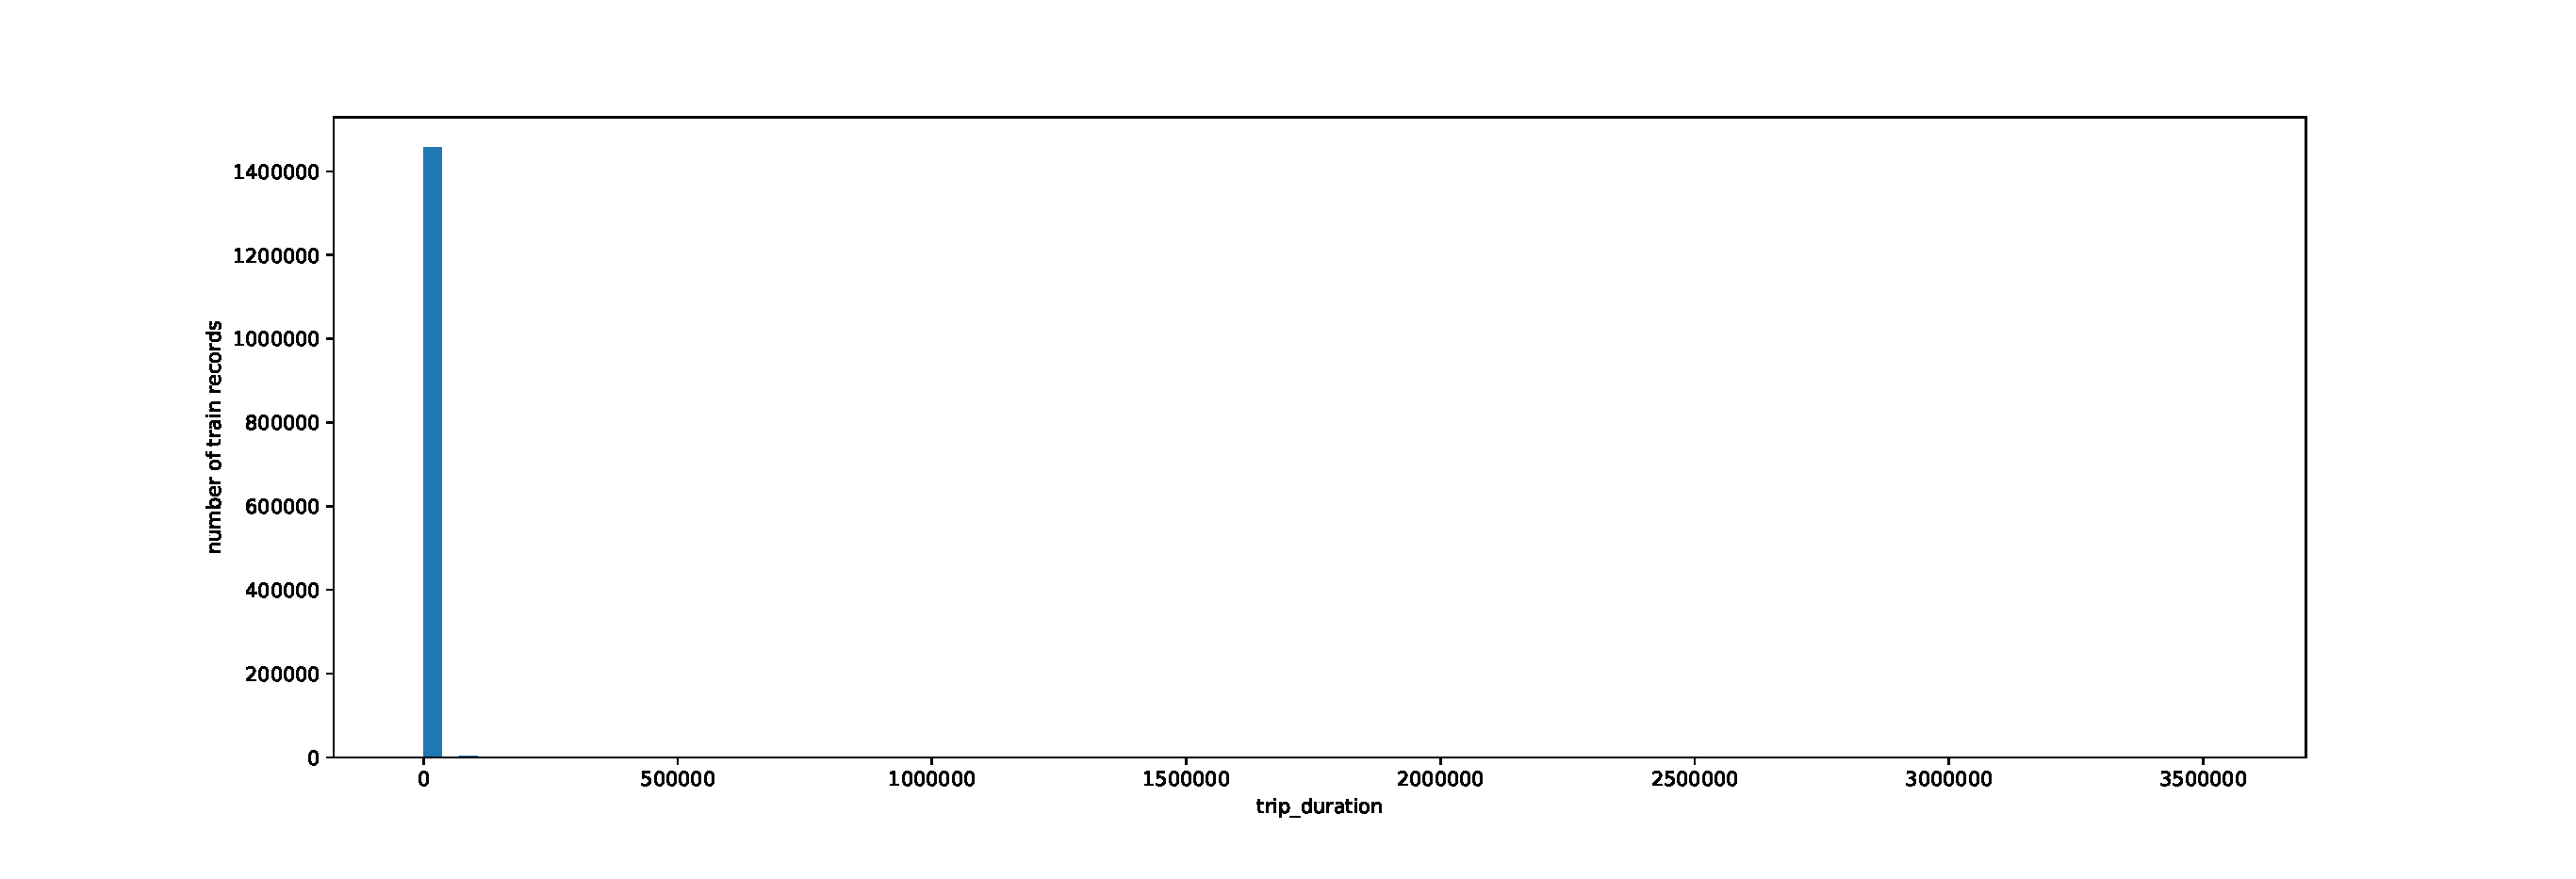
\includegraphics[width=1.0\textwidth]{figure//fig-1.eps}\\
  \caption{Trip-duration}\label{fig:demical}
\end{figure}


%%==========================================================================================
\begin{note}
Based on the above example,
I will compare the differences
between outlying aspects mining and outlier detection.

Outlying aspects mining aims to
explain the distinctive aspects of the query object.
The query object may or may not be an outlier.
In contrast,
Outlier detection aims to discover all possible
outlying objects in the dataset.
Without explaining how and why they are different.

Let's go back to the NBA example,
in that example,
the output of the outlying aspects mining may be
a combination of four features,
but the output of the outlier detection may be any of those five players.
\end{note}
%%==========================================================================================

\end{slide}
%%
%%==========================================================================================



%%
%%==========================================================================================


\section{Feature Engineering}


%%==========================================================================================
%%

%%==========================================================================================

\begin{slide}{Data Preprocessing}

\begin{table}[]
\setlength{\abovecaptionskip}{0pt}
\setlength{\belowcaptionskip}{10pt}
\centering
\caption{Number of non empty samples and field type of each feature}
\begin{tabular}{cccc}
\hline
\textbf{} & \textbf{Column}       & \textbf{Non-Null Count} & \textbf{Dtype} \\
\hline
0         & id                    & 1458644 non-null        & object         \\
1         & vendor\_id            & 1458644 non-null        & int64          \\
2         & pickup\_datetime      & 1458644 non-null        & object         \\
3         & dropoff\_datetime     & 1458644 non-null        & object         \\
4         & passenger\_count      & 1458644 non-null        & int64          \\
5         & pickup\_longitude     & 1458644 non-null        & float64        \\
6         & pickup\_latitude      & 1458644 non-null        & float64        \\
7         & dropoff\_longitude    & 1458644 non-null        & float64        \\
8         & dropoff\_latitude     & 1458644 non-null        & float64        \\
9         & store\_and\_fwd\_flag & 1458644 non-null        & object         \\
10        & trip\_duration        & 1458644 non-null        & int64         \\
\hline
\end{tabular}
\end{table}


%%==========================================================================================
\begin{note}
Based on the above example,
I will compare the differences
between outlying aspects mining and outlier detection.

Outlying aspects mining aims to
explain the distinctive aspects of the query object.
The query object may or may not be an outlier.
In contrast,
Outlier detection aims to discover all possible
outlying objects in the dataset.
Without explaining how and why they are different.
Let's go back to the NBA example,
in that example,
the output of the outlying aspects mining may be
a combination of four features,
but the output of the outlier detection may be any of those five players.
\end{note}
%%==========================================================================================

\end{slide}
%%
%%==========================================================================================

%%==========================================================================================
%%
\begin{slide}[toc=,bm=]{Data Preprocessing}

\begin{itemize}
\item
Analyze outliers:
\begin{itemize}
\item
Select an appropriate \textcolor{orange}{trip-duration} range according to longitude and latitude, and delete the interference data.

\item
According to the analysis, select the data with \textcolor{orange}{trip-duration} less than 1 million, and delete the remaining data.
\end{itemize}
\end{itemize}



%%==========================================================================================
\begin{note}
However,
there is such a phenomenon in real life.
Doctors desire to identify the characteristics between
a group of cancer patients and normal people.
NBA coaches are passionate about exploring the obvious strengths and
weaknesses of the team compared with other teams.

Based on such a phenomenon in the real life,
we proposed the concept of group outlying aspects mining.
\end{note}
%%==========================================================================================

\end{slide}

%%
%%==========================================================================================

%%==========================================================================================
%%
\begin{slide}[toc=,bm=]{Data Preprocessing}

\begin{itemize}
\item
Analyze outliers:
\begin{itemize}
\item
Delete data with \textcolor{orange}{passenger-count} of 0.
\end{itemize}
\end{itemize}

\begin{figure}
  \centering
  \selectcolormodel{rgb}
  %\missingfigure{Testing.}
   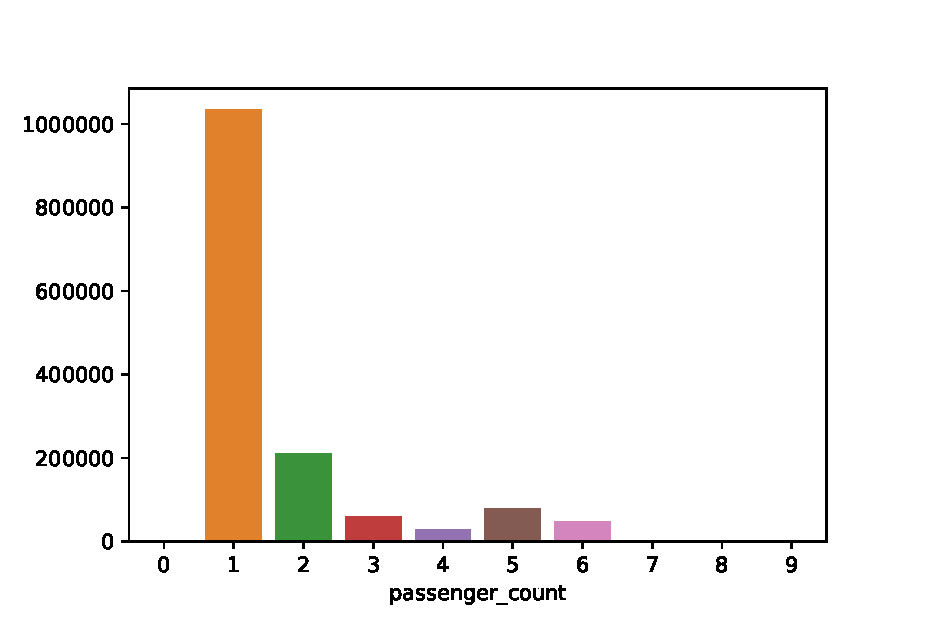
\includegraphics[width=0.5\textwidth]{figure//fig-2.eps}\\
  \caption{Impact of Embarked on Survival}\label{fig:demical}
\end{figure}




%%==========================================================================================
\begin{note}
However,
there is such a phenomenon in real life.
Doctors desire to identify the characteristics between
a group of cancer patients and normal people.
NBA coaches are passionate about exploring the obvious strengths and
weaknesses of the team compared with other teams.

Based on such a phenomenon in the real life,
we proposed the concept of group outlying aspects mining.
\end{note}
%%==========================================================================================

\end{slide}

%%
%%==========================================================================================



%%==========================================================================================
%%
\begin{slide}[toc=,bm=]{Data Preprocessing}

\begin{itemize}
\item
\textcolor{orange}{store-and-fwd-flag} column: string to numeric
\end{itemize}

\centering
\begin{figure}[htbp]
    \centering
    \subfigure[a]{
        \selectcolormodel{rgb}
        %\missingfigure[figwidth=5.5cm]{Test.}
        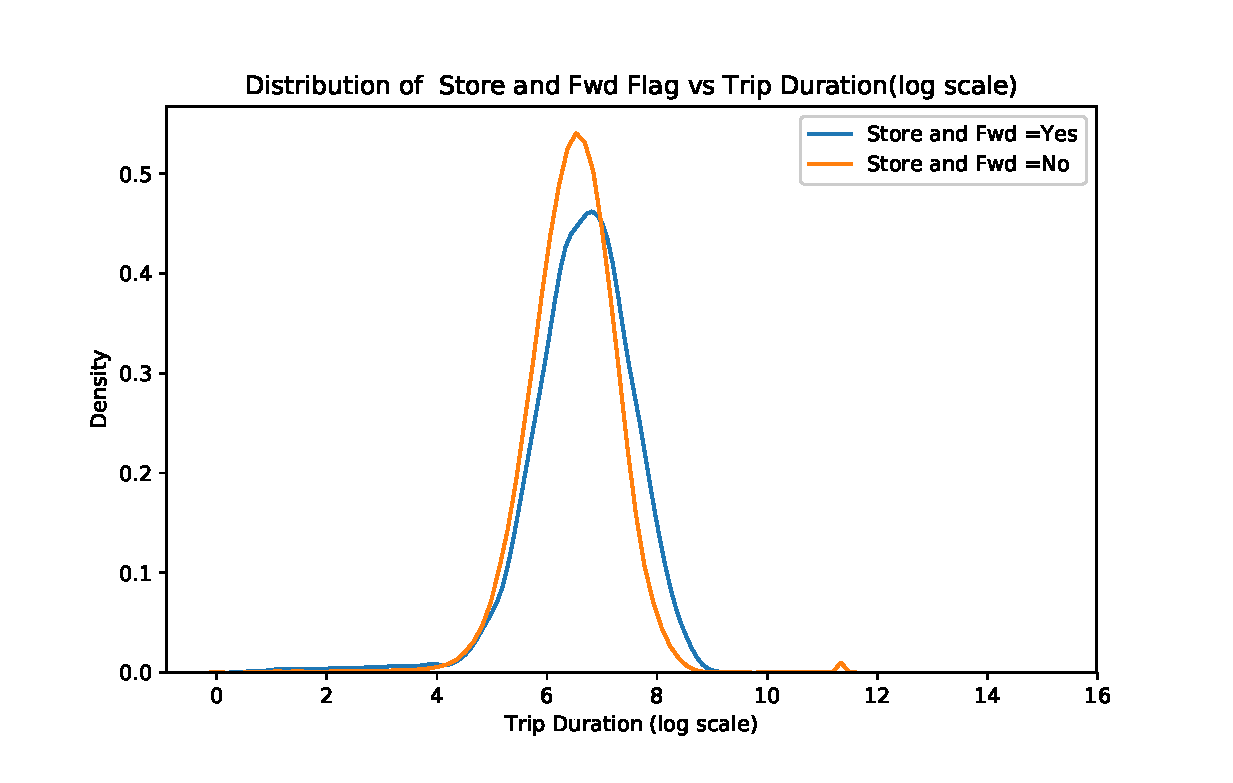
\includegraphics[width=0.35\textwidth]{figure//fig-3.eps}
        \label{fig:fre-dis-f1}
    }
    \subfigure[b]{
        \selectcolormodel{rgb}
        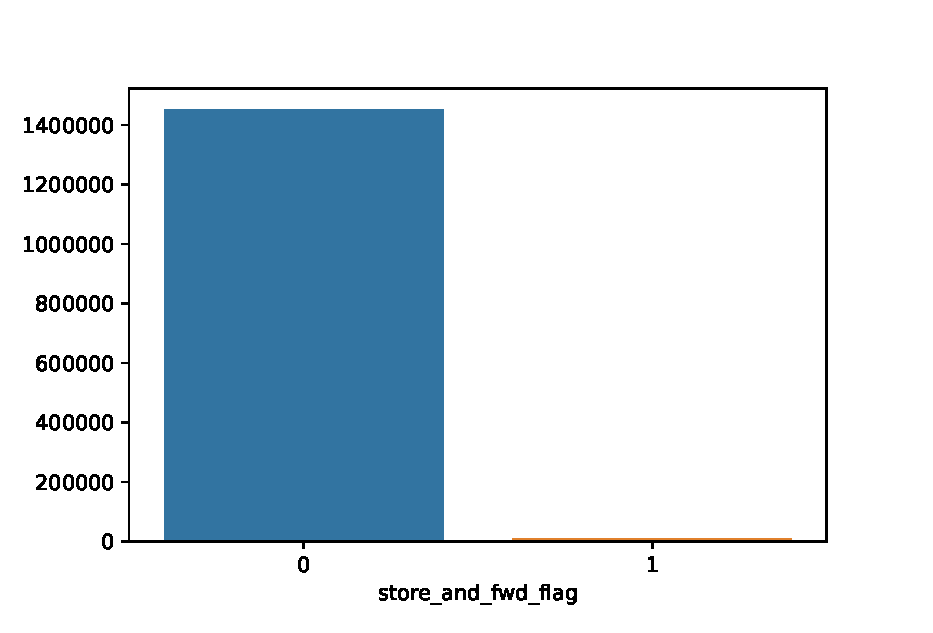
\includegraphics[width=0.35\textwidth]{figure//fig-4.eps}
        \label{fig:fre-dis-f2}
    }
    \caption{Store-and-fwd-flag}
    \label{fig:fre-dis-each-feature}
\end{figure}
\centering



%%==========================================================================================
\begin{note}
However,
there is such a phenomenon in real life.
Doctors desire to identify the characteristics between
a group of cancer patients and normal people.
NBA coaches are passionate about exploring the obvious strengths and
weaknesses of the team compared with other teams.

Based on such a phenomenon in the real life,
we proposed the concept of group outlying aspects mining.
\end{note}
%%==========================================================================================

\end{slide}

%%
%%==========================================================================================


%%==========================================================================================
%%
\begin{slide}{Feature Filtering}

\begin{itemize}
\item
Datetime: object->datetime-> hour, day of week, month
\end{itemize}


\begin{table}[]
\setlength{\abovecaptionskip}{0pt}
\setlength{\belowcaptionskip}{10pt}
\centering
\caption{Data after time processing}
\begin{tabular}{ccccc}
\hline
\textbf{}  & \textbf{pickup\_datetime} & \textbf{day\_of\_week} & \textbf{hour\_of\_the\_day} & \textbf{month} \\
\hline
\textbf{0} & 2016-03-14 17:24:55       & 1                      & 17                          & 3              \\
\textbf{1} & 2016-06-12 00:43:35       & 7                      & 0                           & 6              \\
\textbf{2} & 2016-01-19 11:35:24       & 2                      & 11                          & 1              \\
\textbf{3} & 2016-04-06 19:32:31       & 3                      & 19                          & 4              \\
\textbf{4} & 2016-03-26 13:30:55       & 6                      & 13                          & 3           \\
\hline
\end{tabular}
\end{table}


%%==========================================================================================
\begin{note}
However,
there is such a phenomenon in real life.
Doctors desire to identify the characteristics between
a group of cancer patients and normal people.
NBA coaches are passionate about exploring the obvious strengths and
weaknesses of the team compared with other teams.

Based on such a phenomenon in the real life,
we proposed the concept of group outlying aspects mining.
\end{note}
%%==========================================================================================

\end{slide}

%%
%%==========================================================================================

%%==========================================================================================
%%
\begin{slide}[toc=,bm=]{Feature Filtering}

\begin{itemize}
\item
\textcolor{orange}{Lat-long} to distance by haversine function.
\end{itemize}

\begin{table}[]
\setlength{\abovecaptionskip}{0pt}
\setlength{\belowcaptionskip}{10pt}
\centering
\caption{Data after distance processing}
\resizebox{\textwidth}{!}{
\begin{tabular}{cccccc}
\hline
\textbf{}  & \textbf{pickup\_longitude} & \textbf{pickup\_latitude} & \textbf{dropoff\_longitude} & \textbf{dropoff\_latitude} & {\color[HTML]{FE0000} \textbf{distance}} \\
\hline
\textbf{0} & -73.982155                 & 40.767937                 & -73.964630                  & 40.765602                  & 1.498521                                 \\
\textbf{1} & -73.980415                 & 40.738564                 & -73.999481                  & 40.731152                  & 1.805507                                 \\
\textbf{2} & -73.979027                 & 40.763939                 & -74.005333                  & 40.710087                  & 6.385098                                 \\
\textbf{3} & -74.010040                 & 40.719971                 & -74.012268                  & 40.706718                  & 1.485498                                 \\
\textbf{4} & -73.973053                 & 40.793209                 & -73.972923                  & 40.782520                  & 1.188588              \\
\hline
\end{tabular}}
\end{table}

%%==========================================================================================
\begin{note}
However,
there is such a phenomenon in real life.
Doctors desire to identify the characteristics between
a group of cancer patients and normal people.
NBA coaches are passionate about exploring the obvious strengths and
weaknesses of the team compared with other teams.

Based on such a phenomenon in the real life,
we proposed the concept of group outlying aspects mining.
\end{note}
%%==========================================================================================

\end{slide}

%%
%%==========================================================================================

%%==========================================================================================
%%
\begin{slide}[toc=,bm=]{Feature Filtering}

\begin{itemize}
\item
Normalization: trip-duration -> \textcolor{orange}{log}(trip-duration)
\end{itemize}

\begin{figure}
  \centering
  \selectcolormodel{rgb}
  %\missingfigure{Testing.}
   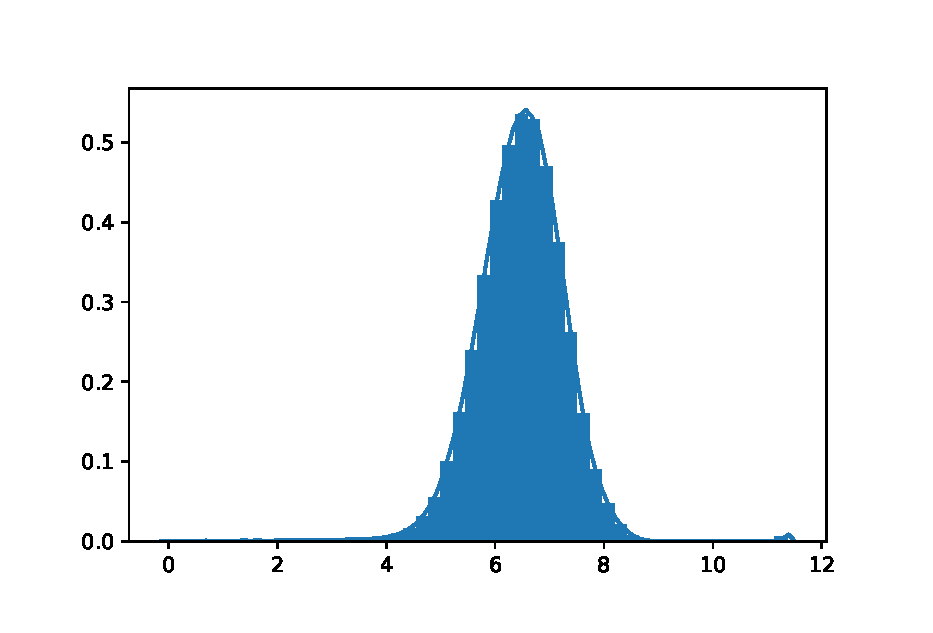
\includegraphics[width=0.5\textwidth]{figure//fig-5.eps}\\
  \caption{Trip-duration}\label{fig:demical}
\end{figure}


%%==========================================================================================
\begin{note}
However,
there is such a phenomenon in real life.
Doctors desire to identify the characteristics between
a group of cancer patients and normal people.
NBA coaches are passionate about exploring the obvious strengths and
weaknesses of the team compared with other teams.

Based on such a phenomenon in the real life,
we proposed the concept of group outlying aspects mining.
\end{note}
%%==========================================================================================

\end{slide}

%%
%%==========================================================================================


%%==========================================================================================
%%
\begin{slide}[toc=,bm=]{Feature Filtering}

\begin{itemize}
\item
The final data result after deleting invalid data:
\end{itemize}


\begin{table}[]
\setlength{\abovecaptionskip}{0pt}
\setlength{\belowcaptionskip}{10pt}
\setlength{\tabcolsep}{10pt} % Default value: 6pt
\renewcommand{\arraystretch}{1.5} % Default value: 1
\centering
\caption{Dataset description}
\resizebox{\textwidth}{!}{
\begin{tabular}{cccccccc}
\hline
\textbf{}  & \textbf{vendor\_id} & \textbf{passenger\_count} & \textbf{store\_and\_fwd\_flag} & \textbf{day\_of\_week} & \textbf{hour\_of\_the\_day} & \textbf{month} & \textbf{distance} \\
\hline
\textbf{0} & 2                   & 1                         & 0                              & 1                      & 17                          & 3              & 1.498521          \\
\textbf{1} & 1                   & 1                         & 0                              & 7                      & 0                           & 6              & 1.805507          \\
\textbf{2} & 2                   & 1                         & 0                              & 2                      & 11                          & 1              & 6.385098          \\
\textbf{3} & 2                   & 1                         & 0                              & 3                      & 19                          & 4              & 1.485498          \\
\textbf{4} & 2                   & 1                         & 0                              & 6                      & 13                          & 3              & 1.188588      \\
\hline
\end{tabular}}
\end{table}

%%==========================================================================================
\begin{note}
However,
there is such a phenomenon in real life.
Doctors desire to identify the characteristics between
a group of cancer patients and normal people.
NBA coaches are passionate about exploring the obvious strengths and
weaknesses of the team compared with other teams.

Based on such a phenomenon in the real life,
we proposed the concept of group outlying aspects mining.
\end{note}
%%==========================================================================================
\end{slide}

%%
%%==========================================================================================





%%==========================================================================================
%%
%page 5
\begin{slide}[toc=,bm=]{Feature Filtering}

\begin{itemize}
\item
Feature relationship heatmap
\end{itemize}

\begin{figure}
  \centering
  \selectcolormodel{rgb}
  %\missingfigure{Testing.}
   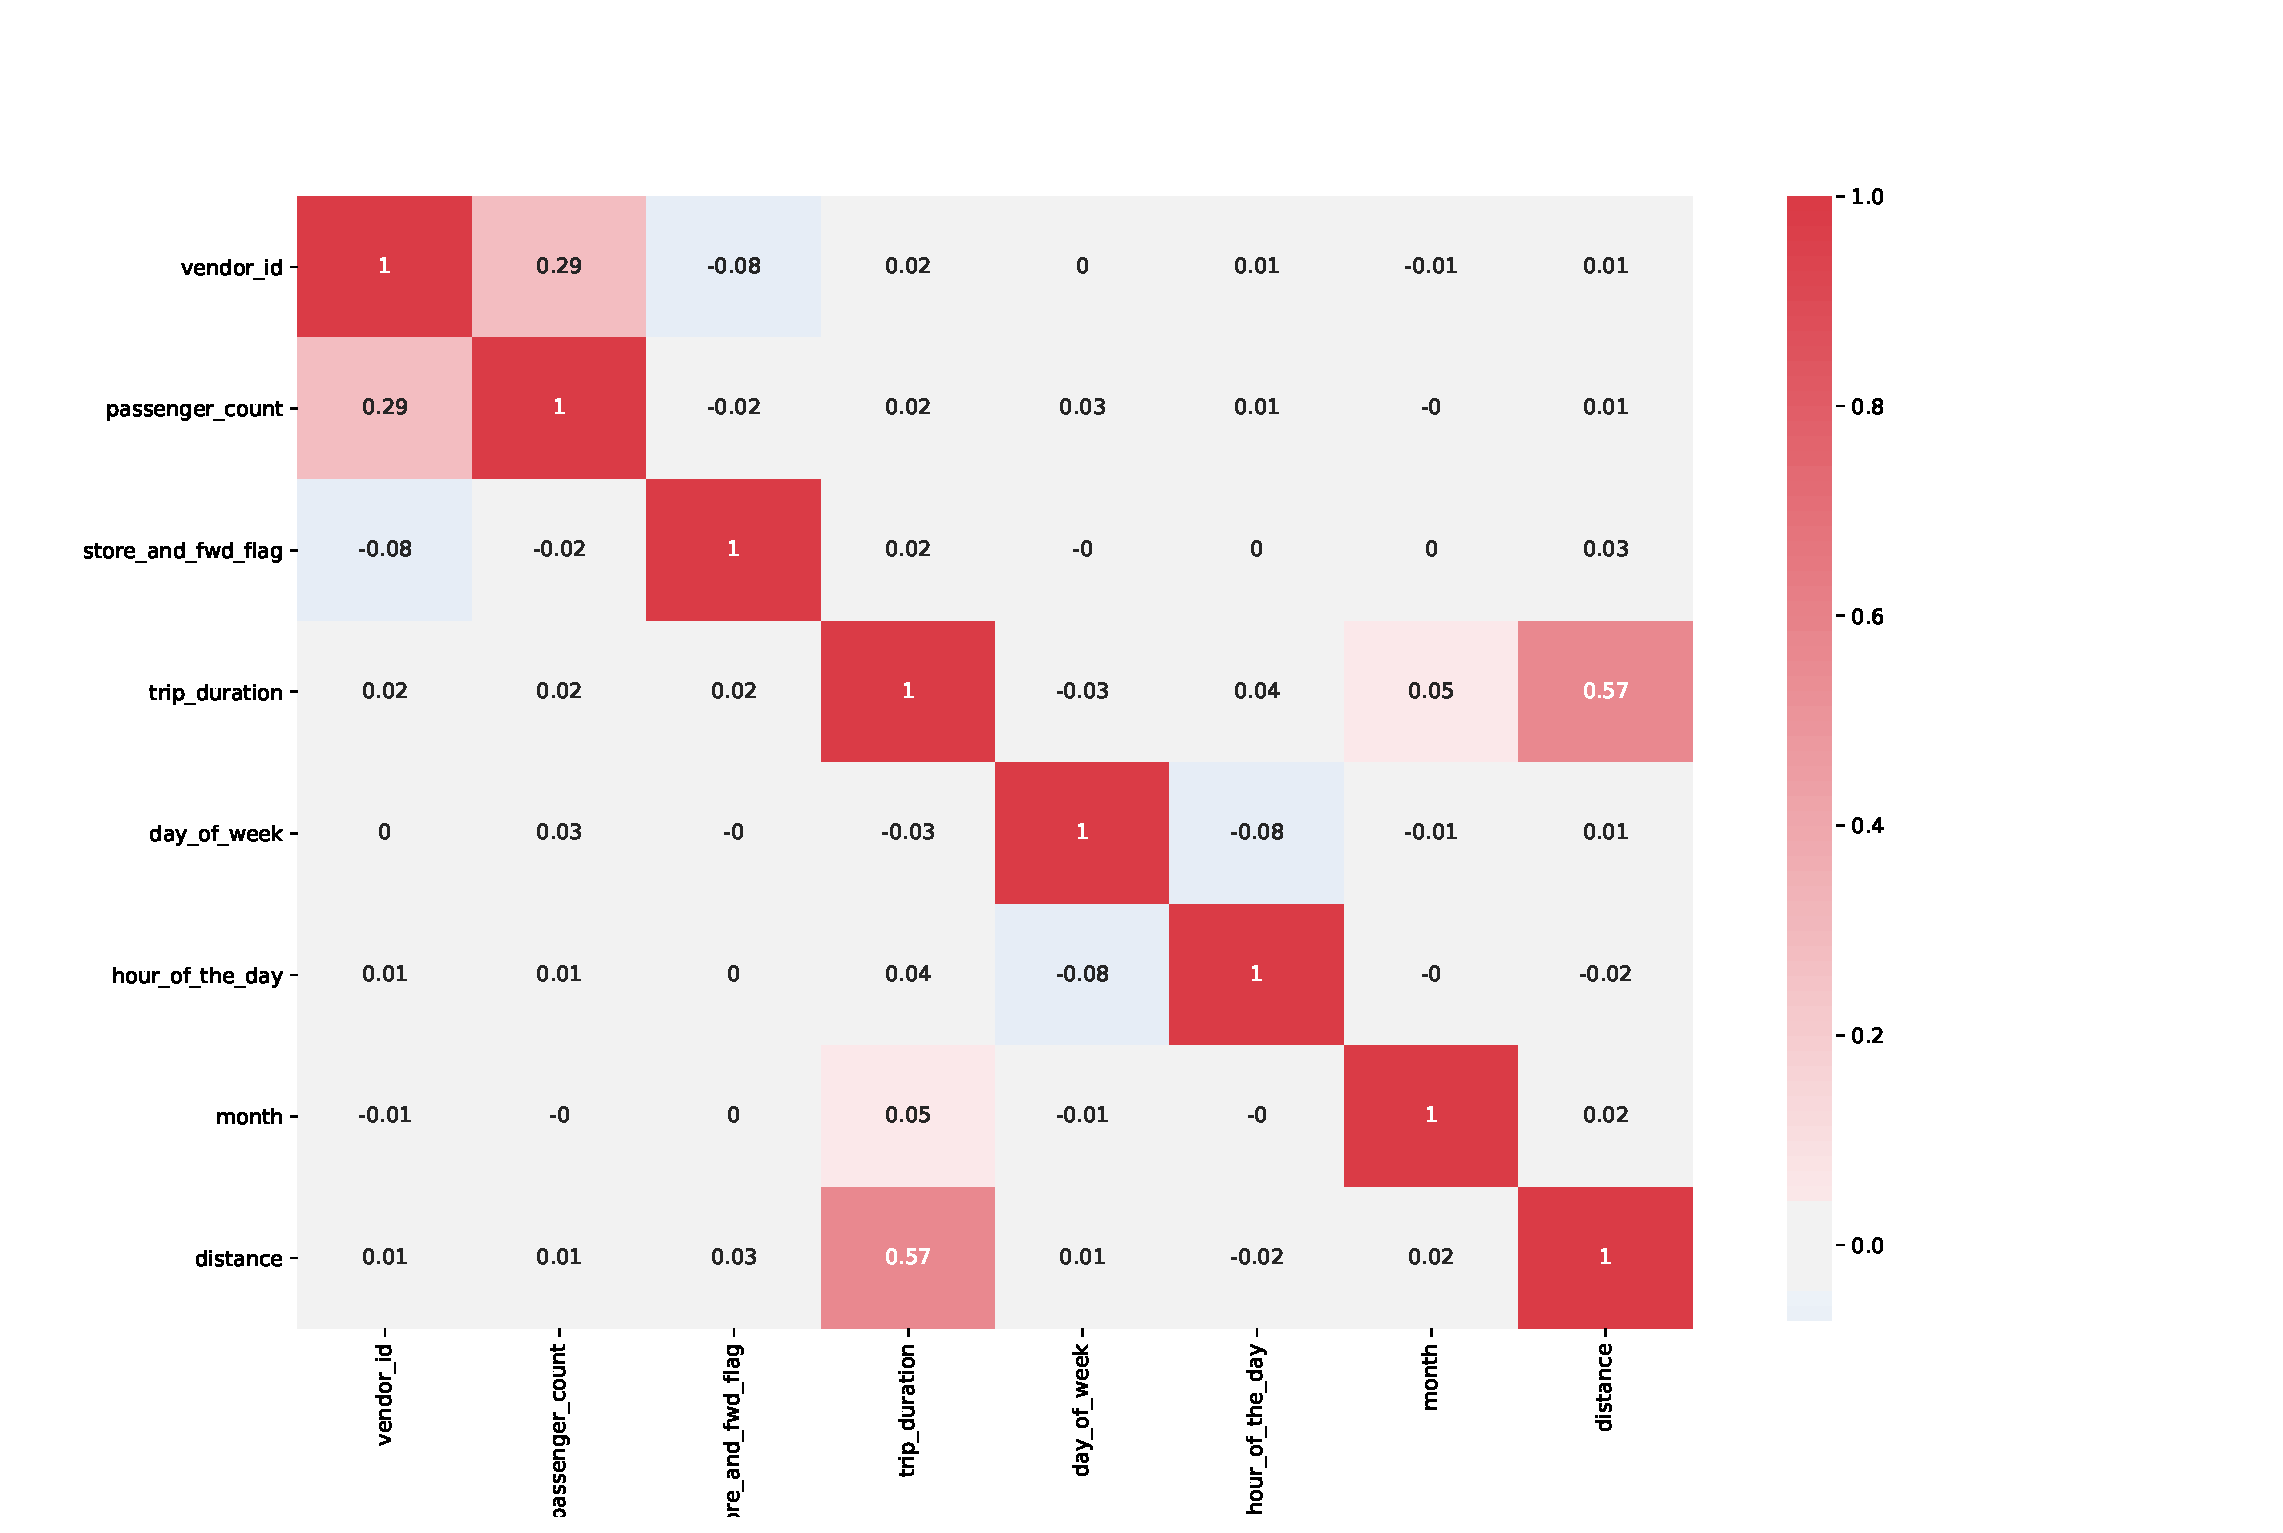
\includegraphics[width=0.5\textwidth]{figure//fig-6.eps}\\
  \caption{Feature relationship diagram}\label{fig:demical}
\end{figure}


%%==========================================================================================
\begin{note}
However,
there is such a phenomenon in real life.
Doctors desire to identify the characteristics between
a group of cancer patients and normal people.
NBA coaches are passionate about exploring the obvious strengths and
weaknesses of the team compared with other teams.

Based on such a phenomenon in the real life,
we proposed the concept of group outlying aspects mining.
\end{note}
%%==========================================================================================

\end{slide}

%%
%%==========================================================================================

%%==========================================================================================
%%
\begin{slide}[toc=,bm=]{Feature Filtering}

\begin{itemize}
\item
Visual analysis of important features
\end{itemize}


\begin{figure}[htbp]
    \centering
    \subfigure[vendor-id]{
        \selectcolormodel{rgb}
        %\missingfigure[figwidth=5.5cm]{Test.}
        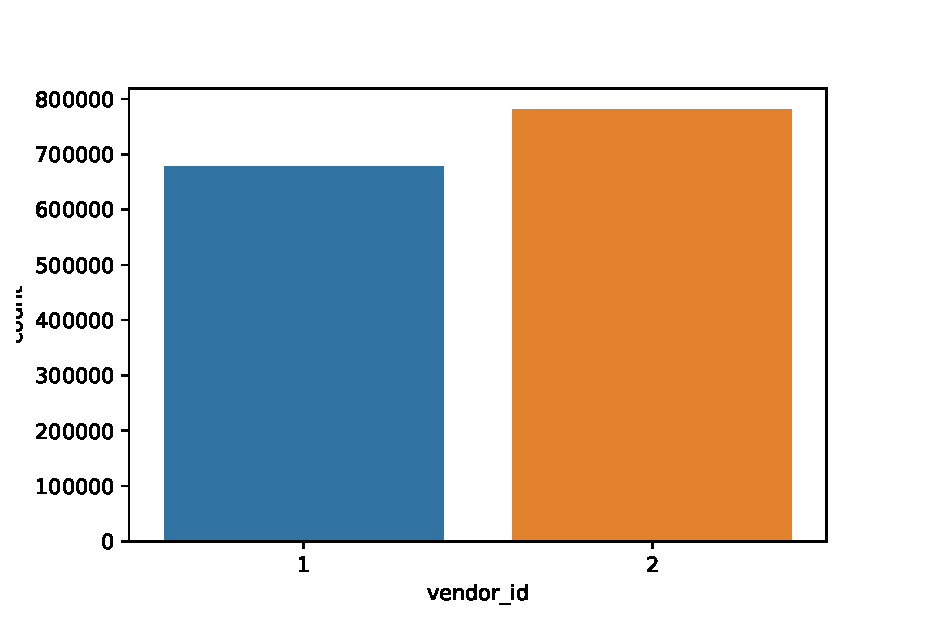
\includegraphics[width=0.35\textwidth]{figure//fig-7.eps}
        \label{fig:fre-dis-f1}
    }
    \subfigure[day-of-week]{
        \selectcolormodel{rgb}
        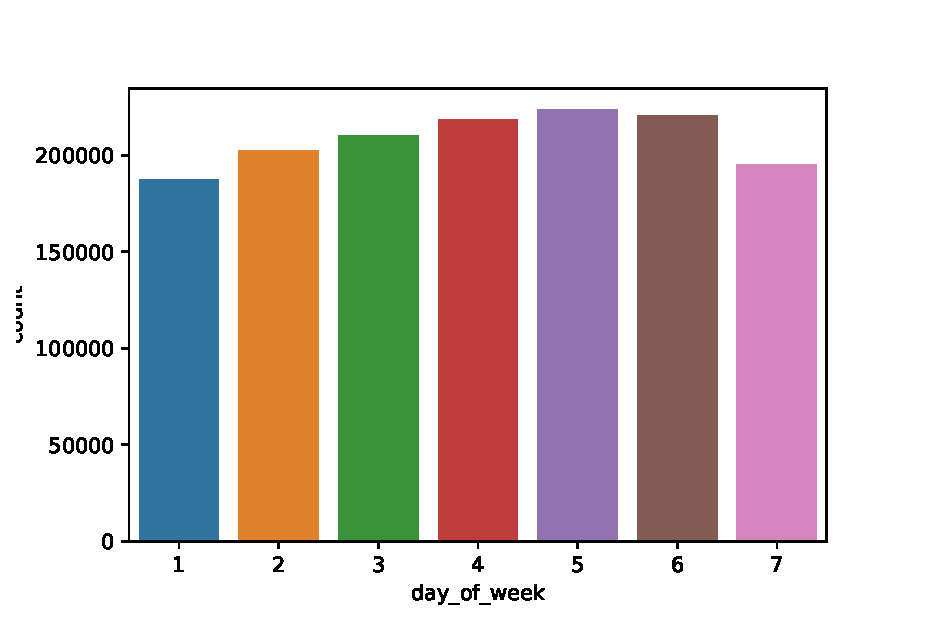
\includegraphics[width=0.35\textwidth]{figure//fig-8.eps}
        \label{fig:fre-dis-f2}
    }
    \caption{Feature analysis}
    \label{fig:fre-dis-each-feature}
\end{figure}


%%==========================================================================================
\begin{note}
In order to tackle the above issues,
GOAM algorithm is involved.

Let's have a look at the framework of this algorithm.
The first step is to use the histogram to represent the group features
based on all individuals in the group.

Following that,
we utilize the earth mover distances to measure the
outlying degree between groups.
This is the second step:
outlying degree scoring.

The last step is to identify the outlying aspects.

\end{note}
%%==========================================================================================

\end{slide}
%%
%%==========================================================================================



%%==========================================================================================
%%
\begin{slide}[toc=,bm=]{Feature Filtering}

\begin{itemize}
\item
Visual analysis of important features
\end{itemize}


\begin{figure}[htbp]
    \centering
    \subfigure[hour-of-the-day]{
        \selectcolormodel{rgb}
        %\missingfigure[figwidth=5.5cm]{Test.}
        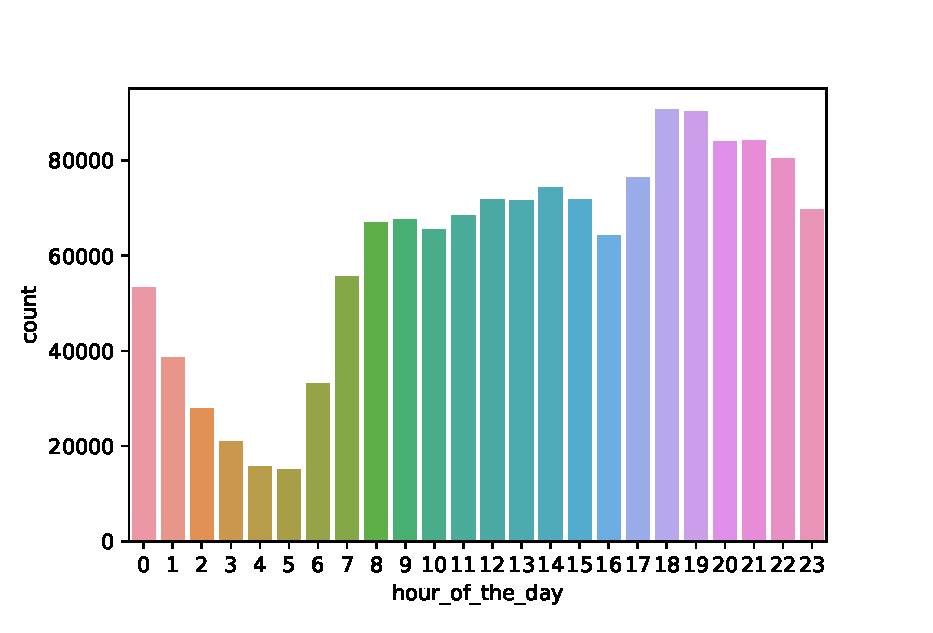
\includegraphics[width=0.35\textwidth]{figure//fig-9.eps}
        \label{fig:fre-dis-f1}
    }
    \subfigure[month]{
        \selectcolormodel{rgb}
        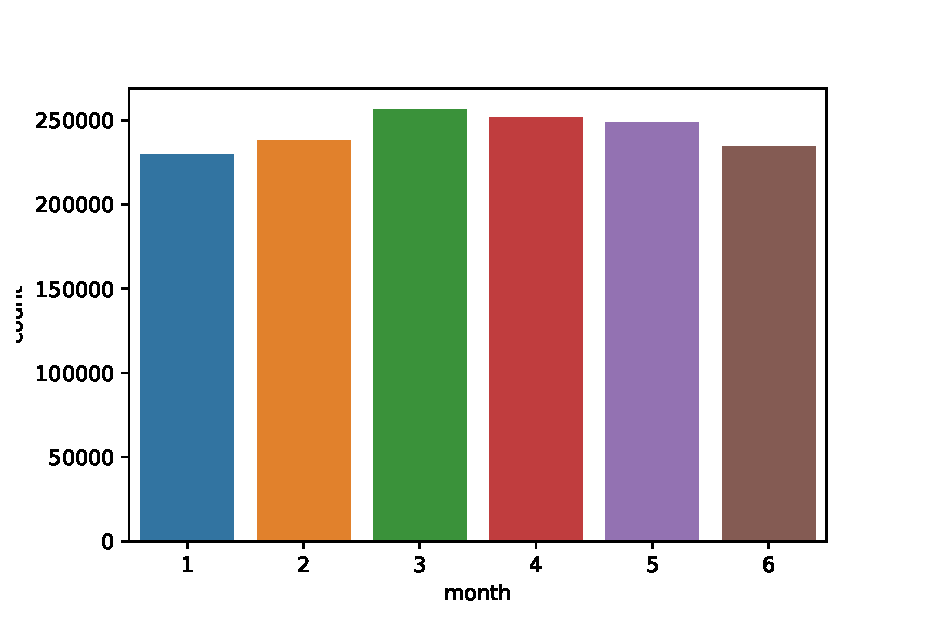
\includegraphics[width=0.35\textwidth]{figure//fig-10.eps}
        \label{fig:fre-dis-f2}
    }
    \caption{Feature analysis}
    \label{fig:fre-dis-each-feature}
\end{figure}


%%==========================================================================================
\begin{note}
In order to tackle the above issues,
GOAM algorithm is involved.

Let's have a look at the framework of this algorithm.
The first step is to use the histogram to represent the group features
based on all individuals in the group.

Following that,
we utilize the earth mover distances to measure the
outlying degree between groups.
This is the second step:
outlying degree scoring.

The last step is to identify the outlying aspects.

\end{note}
%%==========================================================================================

\end{slide}
%%
%%==========================================================================================


%%
%%==========================================================================================


\section{Model introduction}


%%==========================================================================================
%%
%page 10
\begin{slide}{Model introduction}
%Related Work - Outlying Aspects Mining
\begin{itemize}
\item
Five models were selected in this experiment: \textcolor{orange}{LGBMRegressor, LinearRegression, DecisionTreeRegressor}.

\item
The division ratio of training set and test set is set to \textcolor{orange}{0.3}.

\end{itemize}




%%==========================================================================================
\begin{note}
Let me introduce two existing methods:
Feature selection and score-and-search.

For feature selection,
the query point can be regarded as positive class and
the rest of the data can be regarded as negative class,
selected the features that best distinguish the two classes.

The advantages of this method are easy to operate,
and it's able to resolve dimensionality bias.
However, it has some drawbacks.
Firstly,
positive and negative classes are Not balanced,
secondly,
it can't quantify the outlying degree correctly.
Most importantly,
it doesn't identify group outlying aspects.
\end{note}
%%==========================================================================================

\end{slide}
%%
%%==========================================================================================






%%==========================================================================================


\section{Evaluation Results and Analysis}


%%==========================================================================================


%%==========================================================================================
%%
\begin{slide}{Experimental result}

\begin{center}
\begin{itemize}

\item
\smallskip
\large
%{$Accuracy = \frac{P}{T}$ \\
${MSE = \frac{1}{m}{\sum\limits_{i = 1}^m {\left( {f\left( {{x_i}} \right) - {y_i}} \right)} ^2}}$

\item
${MAE = \frac{1}{N}\sum\limits_{i = 1}^N {\left| {{y_i} - f\left( {{x_i}} \right)} \right|} }$

\item
${RMSE = \sqrt {\frac{1}{N}\sum\limits_{i = 1}^N {{{\left( {{y_i} - f\left( {{x_i}} \right)} \right)}^2}} } }$

\end{itemize}
\end{center}


%%==========================================================================================
\begin{note}
Now, let me specifically explain what each step means.
The first step is group feature extraction.
we can take one group extraction as an example.

We suppose to use $f_1$, $f_2$, $f_3$ to represent three features of $G_q$.
The values of $f_1$ are {$x_1$, $x_2$, $x_3$, $x_4$} and so on.
And the values of $f_2$ are {$y_2$, $y_2$, $y_1$, $x_2$} and so on.

For feature $f_1$,
we use the histogram to illustrate feature $f_1$ after
counting the frequency of each value,
as show in figure 6 (a).

\begin{table}
\setlength{\abovecaptionskip}{0pt}
\setlength{\belowcaptionskip}{10pt}
\centering
\caption{Synthetic Dataset and Ground Truth}

\begin{tabular}{p{2.8cm}p{0.9cm}p{0.9cm}p{0.9cm}p{0.9cm}p{0.9cm}p{0.9cm}p{0.9cm}p{0.9cm}}
\hline
  % after \\: \hline or \cline{col1-col2} \cline{col3-col4} ...
  Query group  & $\mathbf{F_1}$ & $\mathbf{F_2}$ & $F_3$ & $\mathbf{F_4}$ & $F_5$ & $F_6$ & $F_7$ & $F_8$\\
\hline
  $i_1$   & \bf{10} & \bf{8}  & 9  & \bf{7}  & 7 & 6 & 6  & 8\\
  $i_2$   & \bf{9}  & \bf{9}  & 7  & \bf{8}  & 9 & 9 & 8  & 9\\
  $i_3$   & \bf{8}  & \bf{10} & 8  & \bf{9}  & 6 & 8 & 7  & 8\\
  $i_4$   & \bf{8}  & \bf{8}  & 6  & \bf{7}  & 8 & 8 & 6  & 7\\
  $i_5$   & \bf{9}  & \bf{9}  & 9  & \bf{7}  & 7 & 7 & 8  & 8\\
  $i_6$   & \bf{8}  & \bf{10} & 8  & \bf{8}  & 6 & 6 & 8  & 7\\
  $i_7$   & \bf{9}  & \bf{9}  & 7  & \bf{9}  & 8 & 8 & 8  & 7\\
  $i_8$   & \bf{10} & \bf{9}  & 10 & \bf{7}  & 7 & 7 & 7  & 7\\
  $i_9$   & \bf{9}  & \bf{10} & 8  & \bf{8}  & 7 & 6 & 7  & 7\\
  $i_{10}$& \bf{9}  & \bf{9}  & 7  & \bf{7}  & 7 & 8 & 8  & 8\\
\hline
\end{tabular}
\end{table}

Similarly,

\begin{table}[tb]
\setlength{\abovecaptionskip}{0pt}
\setlength{\belowcaptionskip}{10pt}
\centering
\caption{Collected data of Brooklyn Nets Team}

\begin{tabular}{p{0.9cm}p{0.9cm}p{0.9cm}p{0.9cm}p{0.9cm}p{0.9cm}p{0.9cm}p{0.9cm}p{0.9cm}p{0.9cm}p{0.9cm}p{0.9cm}}
\hline
  Pts & FGA & FG\% & 3FA & 3PT\% & FTA & FT\% & Reb & Ass & To & Stl & Blk \\
\hline
  18   & 12    & 42 &2.00 & 50 & 7.00 & 100& 0& 4& 3& 0& 0 \\
  15.7 & 14.07 & 41 &5.45 & 32 & 3.05 & 75 & 3.98& 5.1& 2.98& 0.69& 0.36\\
  14.5 & 11.1  & 47 &0.82 & 26 & 4.87 & 78 & 6.82& 2.4& 1.74& 0.92& 0.66 \\
  13.5 & 10.8  & 42 &5.37 & 37 & 3.38 & 77 & 6.66& 2& 1.38& 0.83& 0.42 \\
  12.7 & 10.59 & 39 &5.36 & 33 & 3.37 & 82 & 3.24& 6.6& 1.56& 0.89& 0.31 \\
  12.6 & 10.93 & 40 &6.94 & 37 & 1.70 & 84 & 4.27& 1.5& 1.06& 0.61& 0.44 \\
  12.2 & 10.39 & 44 &3.42 & 35 & 2.70 & 72 & 3.79& 4.1& 2.15& 1.12& 0.32 \\
  10.6 & 7.85  & 49 &4.51 & 41 & 1.35 & 83 & 3.34& 1.6& 1.15 & 0.45& 0.24 \\
\hline
\end{tabular}
\end{table}

we can also extract other features of the group
according to feature $f_1$.
\end{note}
%%==========================================================================================

\end{slide}
%%
%%==========================================================================================


%%==========================================================================================
%%
\begin{slide}[toc=,bm=]{Experimental result}



\begin{table}[]
\setlength{\abovecaptionskip}{0pt}
\setlength{\belowcaptionskip}{10pt}
\setlength{\tabcolsep}{10pt} % Default value: 6pt
\renewcommand{\arraystretch}{1.5} % Default value: 1
\centering
\caption{The experiment result on synthetic dataset}
\begin{tabular}{cccc}
\hline
\textbf{Model} & \textbf{LGBMRegressor}      & \textbf{LinearRegression} & \textbf{DecisionTreeRegressor} \\
\hline
R2\_score      & 0.66                        & 0.35                      & 0.3                            \\
MSE            & {\color[HTML]{FE0000} 0.22} & 0.42                      & 0.45                           \\
MAE            & {\color[HTML]{FE0000} 0.32} & 0.46                      & 0.46                           \\
RMSE           & {\color[HTML]{FE0000} 0.47} & 0.65                      & 0.67  \\
\hline
\end{tabular}
\end{table}

%%==========================================================================================
\begin{note}
Now, let me specifically explain what each step means.
The first step is group feature extraction.
we can take one group extraction as an example.

We suppose to use $f_1$, $f_2$, $f_3$ to represent three features of $G_q$.
The values of $f_1$ are {$x_1$, $x_2$, $x_3$, $x_4$} and so on.
And the values of $f_2$ are {$y_2$, $y_2$, $y_1$, $x_2$} and so on.

For feature $f_1$,
we use the histogram to illustrate feature $f_1$ after
counting the frequency of each value,
as show in figure 6 (a).


Similarly,

we can also extract other features of the group
according to feature $f_1$.
\end{note}
%%==========================================================================================

\end{slide}
%%
%%==========================================================================================



%%==========================================================================================


\section{Conclusion}

%%==========================================================================================
%%
\begin{slide}{Conclusion}
\begin{itemize}
\item
\smallskip
The competition dataset is based on the 2016 NYC Yellow Cab trip record data made available in Big Query on Google Cloud Platform. The real data set is helpful to verify the authenticity and reliability of the test results;

\item
\smallskip
In this project, the effects of 3 baseline models on 4 evaluation indexes are compared. Finally, it is found that the prediction effect of LGBMRegressor model is the best as a whole;

\item
\smallskip
By analyzing this data set, we can not only predict the travel time of passengers, but also mine more detailed information about urban travel behavior. For example, you can analyze which areas in which periods of time are more prone to orders, and where people generally go from. This is an effective data for rental scheduling. It can be inferred from the abnormal value brought by the blizzard that the weather is closely related to the order quantity. According to the weather data corresponding to the date, the impact of the weather and the order quantity can be further analyzed. Combined with the location data, it can also analyze which areas are greatly affected by the weather, etc.

\end{itemize}



%%==========================================================================================
\begin{note}
In conclusion,
we firstly formalized the problem of
group outlying aspects mining,

Then proposed a novel method GOAM algorithm to address the problem of
group outlying aspects mining,
and the proposed method use pruning to reduce time complexity
while identifying the suitable set of outlying features for the interested group.

Thank you and any question?
\end{note}
%%==========================================================================================

\end{slide}
%%
%%==========================================================================================




%%==========================================================================================
%
\begin{slide}[toc=,bm=]{Questions?}
\begin{center}
\begin{figure}
    \animategraphics[autoplay, loop, height=0.4\textheight]{5}{./graphics//gif//question//q_}{1}{30}
\end{figure}
\end{center}
\end{slide}
%%
%%==========================================================================================


%%==========================================================================================
% TODO: Contact Page
\begin{wideslide}[toc=,bm=]{Contact Information}
\centering
\vspace{\stretch{1}}
\twocolumn[
lcolwidth=0.35\linewidth,
rcolwidth=0.65\linewidth
]
{
% \centerline{
\includegraphics[scale=.2]{tulip-logo.eps}}
}
{
\vspace{\stretch{1}}
Qin Zhang\\
School of Artificial Intelligence\\
Chongqing Technology and Business University, China
\begin{description}
 \item[\textcolor{orange}{\faEnvelope}] \href{mailto:qzhang@tulip.academy}
 {\textsc{\footnotesize{qzhang@tulip.academy}}}

 \item[\textcolor{orange}{\faHome}] \href{http://www.tulip.org.au}
 {\textsc{\footnotesize{Team for Universal Learning and Intelligent Processing}}}
\end{description}
}
\vspace{\stretch{1}}
\end{wideslide}

\end{document}

\endinput
